% Metamodel: CSP-M
\newcommand{\mcspfragment}{\metaref{CSPFragment}}
\newcommand{\meventsetcspfragment}{\metaref{EventSetCSPFragment}}
\newcommand{\minlinecspfragment}{\metaref{InlineCSPFragment}}
\newcommand{\mprocesscspfragment}{\metaref{ProcessCSPFragment}}
\newcommand{\mcsprefinementproperty}{\metaref{CSPRefinementProperty}}
\newcommand{\mcspprocesssource}{\metaref{CSPProcessSource}}
\newcommand{\mcspcontextsource}{\metaref{CSPContextSource}}


We define \langname{} by defining its
metamodel.  Parts of the metamodel map to various concrete notations (for
instance, sequences map to UML-style sequence diagrams), and have a semantics
in terms of process algebras and other formalisms (\cref{cha:semantics-intro}).

This chapter discusses the top-level metamodel and, in turn, the key concepts
of \langname.

\section{Introduction}\label{ssec:core-metamodel-intro}
\subsection{How to read the rest of this chapter}\label{ssec:core-metamodel-intro-readme}

Each section, except this one,
introduces a group of top-level \langname{}
functionality in a top-down manner.  These sections contain:

\begin{itemize}
\item
	a class diagram representing the Ecore classes, enumerations, and other
	components that make up the group being discussed;
\item
	descriptions of the components being shown in the class diagram;
\item
	where relevant, examples of the components in terms of the concrete
	syntaxes of \langname.
\end{itemize}

\section{Top-level}\label{sec:core-metamodel-top}
% !TEX root=../../robocert.tex
\begin{figure}[htb]
  \centering
  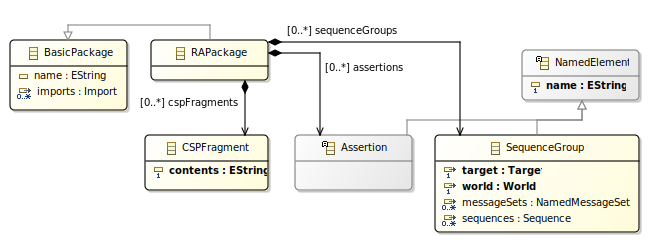
\includegraphics[width=.85\textwidth]{diagrams/Top}
  \caption{Class diagram for the top of the \langname{} metamodel.}
  \label{fig:metamodel-top}
\end{figure}

\Cref{fig:metamodel-top} is the top-level metamodel diagram for \langname.

Each \langname{} script contains an \mrapackage,\footnote{\mrapackage{} stands
  for `RoboStar Assertions package'; we use this name because \mrcpackage{} is
  already used for RoboChart packages.}
which is a type of RoboStar \mbasicpackage.
Each \mrapackage{} can contain zero or more of each of these types of content:

\begin{itemize}
\item
  \msequencegroup:
  a sequence diagram group
  (see \cref{sec:metamodel-sequences});
\item
  \mcspgroup:
  a CSP fragment, currently not bound to a particular process
  \todo{this will change};
\item
  \massertion:
  an assertion
  (see \cref{sec:core-metamodel-assertions}).
\end{itemize}

%%% Local Variables:
%%% mode: latex
%%% TeX-master: "../../robocert"
%%% End:


\section{Assertions}\label{sec:core-metamodel-assertions}
%!TEX root=../robocert.tex
\begin{figure}
	\centering
	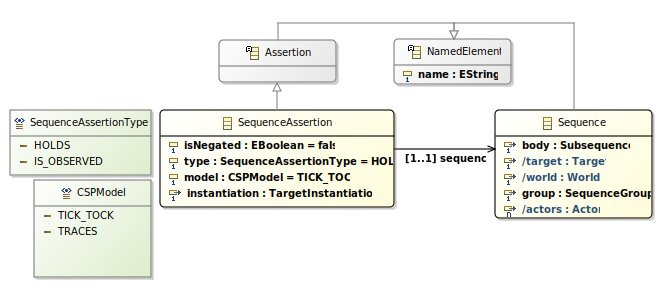
\includegraphics[width=0.7\textwidth]{diagrams/Assertions}
	\caption{Class diagram for the part of the \langname{} metamodel dealing with assertions.}
	\label{fig:metamodel-assertions}
\end{figure}

\Cref{fig:metamodel-assertions} depicts the part of the metamodel concerning
assertions.

\subsection{\massertion}

An \massertion{} is a named assertion statement.  Currently, there is
only one type of assertion: a \msequenceassertion{}.  \todo{This will change
when merging with the existing language, if not sooner.}

\subsection{\msequenceassertion}\label{ssec:metamodel-assertions-sequence}

A \msequenceassertion{} is an assertion about a particular \msequence{} with
respect to its \mtarget.  The \mtarget{} is modified by applying an
assertion-level \mtargetinstantiation, which may fix any constants not bound
by the sequence-level instantiation.  (The default is an empty instantiation,
meaning the target is exactly as specified at the sequence level.)

The specific sequence assertion type comes from the \msequenceassertiontype:
either `sequence holds on target' (refinement), or `sequence is observed on
target' (reverse refinement).  The assertion can be negated.  The choice of
\mcspmodel{} affects how the assertion is checked with CSP tools such as FDR
\todo{the models aren't actually used yet; everything is treated as untimed
traces refinement.  This will change.}

\begin{lstlisting}[style=Example]
assertion A: SequenceName holds           // positive 'holds' SequenceAssertion
assertion B: SequenceName does not hold   // negative 'holds' SequenceAssertion
assertion C: SequenceName is observed     // positive 'is observed' SequenceAssertion
assertion D: SequenceName is not observed // negative 'is observed' SequenceAssertion

assertion E: SequenceName holds with { CONSTANT set to 5 }
// example of SequenceAssertion with custom TargetInstantiation
\end{lstlisting}

%%% Local Variables:
%%% mode: latex
%%% TeX-master: "../robocert"
%%% End:


%%% Local Variables:
%%% mode: latex
%%% TeX-master: "../robocert"
%%% End:
